\documentclass[aspectratio=169]{beamer}
\usetheme{Madrid}
\usecolortheme{seahorse}

\usepackage{tikz}
\usepackage{listings}
\usepackage{booktabs}
\usepackage{amsmath}

\usetikzlibrary{arrows.meta, positioning, shapes.geometric, fit, decorations.pathreplacing}

\lstset{
  language=Python,
  basicstyle=\ttfamily\scriptsize,
  keywordstyle=\color{blue}\bfseries,
  commentstyle=\color{gray},
  stringstyle=\color{red!70!black},
  showstringspaces=false,
  frame=single,
  backgroundcolor=\color{gray!5},
  breaklines=true,
}

\title{ADC Waveform Signal Extraction}
\subtitle{ML Pipeline Overview}
\author{Artur}
\date{\today}

\begin{document}

% ============================================================
\begin{frame}
\titlepage
\end{frame}

% ============================================================
\begin{frame}{Outline}
\tableofcontents
\end{frame}

% ============================================================
\section{Problem Statement}

\begin{frame}{Problem Statement}
\begin{columns}[T]
\column{0.55\textwidth}
\textbf{Goal:} Extract individual signal pulses from noisy ADC waveforms.

\medskip
Given a digitized waveform containing:
\begin{itemize}
  \item 0--6 overlapping signal pulses
  \item Additive Gaussian noise ($\sigma = 0.5$)
  \item DC baseline offset (200 ADC counts)
\end{itemize}

\medskip
Predict:
\begin{enumerate}
  \item \textbf{How many} signals are present (classification)
  \item \textbf{Where and how large} each signal is: $(t_0, A)$ pairs (regression)
\end{enumerate}

\column{0.42\textwidth}
\centering
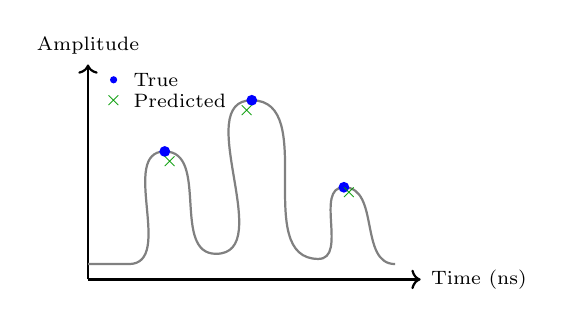
\begin{tikzpicture}[scale=0.65]
  % Axes
  \draw[->, thick] (0,0) -- (6.5,0) node[right] {\scriptsize Time (ns)};
  \draw[->, thick] (0,0) -- (0,4.2) node[above] {\scriptsize Amplitude};
  % Waveform (stylized)
  \draw[gray, thick] (0,0.3) -- (0.8,0.3) to[out=0,in=180] (1.5,2.5)
    to[out=0,in=180] (2.5,0.5) to[out=0,in=180] (3.2,3.5)
    to[out=0,in=180] (4.5,0.4) to[out=0,in=180] (5,1.8)
    to[out=0,in=180] (6,0.3);
  % Signal markers
  \fill[blue] (1.5,2.5) circle (3pt);
  \fill[blue] (3.2,3.5) circle (3pt);
  \fill[blue] (5,1.8) circle (3pt);
  % Predicted markers
  \node[green!60!black, mark size=3pt] at (1.6,2.3) {\scriptsize$\times$};
  \node[green!60!black, mark size=3pt] at (3.1,3.3) {\scriptsize$\times$};
  \node[green!60!black, mark size=3pt] at (5.1,1.7) {\scriptsize$\times$};
  % Legend
  \fill[blue] (0.5,3.9) circle (2pt); \node[right, font=\scriptsize] at (0.7,3.9) {True};
  \node[green!60!black] at (0.5,3.5) {\scriptsize$\times$}; \node[right, font=\scriptsize] at (0.7,3.5) {Predicted};
\end{tikzpicture}
\end{columns}
\end{frame}

% ============================================================
\section{Pipeline Architecture}

\begin{frame}{Pipeline Overview}
\centering
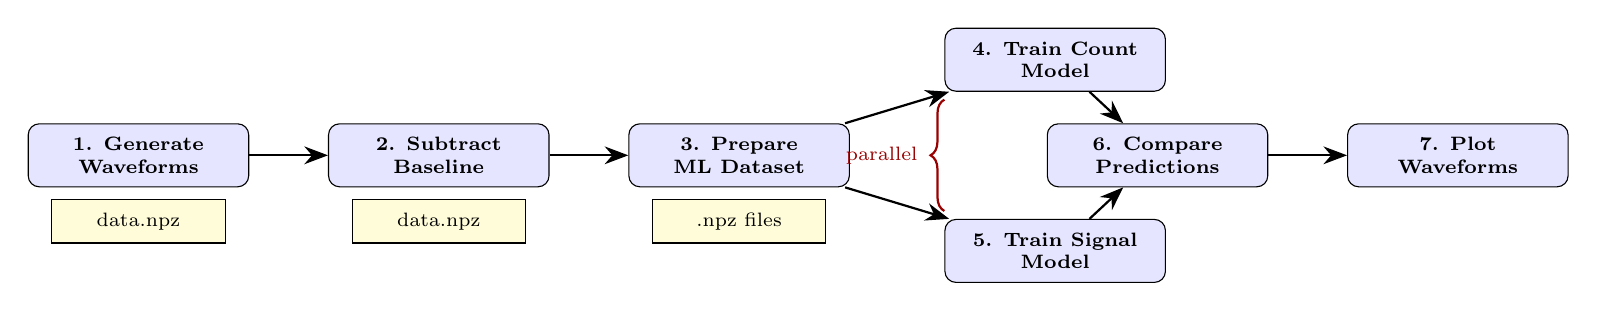
\begin{tikzpicture}[
  node distance=0.6cm and 1.0cm,
  box/.style={rectangle, draw, rounded corners, fill=blue!10,
              minimum width=2.8cm, minimum height=0.8cm, align=center,
              font=\scriptsize\bfseries},
  data/.style={rectangle, draw, fill=yellow!15, minimum width=2.2cm,
               minimum height=0.55cm, align=center, font=\scriptsize},
  arr/.style={-{Stealth[length=3mm]}, thick}
]
  \node[box] (gen)  {1. Generate\\Waveforms};
  \node[box, right=of gen] (base) {2. Subtract\\Baseline};
  \node[box, right=of base] (prep) {3. Prepare\\ML Dataset};

  \node[box, above right=0.4cm and 1.2cm of prep] (count) {4. Train Count\\Model};
  \node[box, below right=0.4cm and 1.2cm of prep] (signal) {5. Train Signal\\Model};

  \node[box, right=2.5cm of prep, yshift=0cm] (compare) {6. Compare\\Predictions};
  \node[box, right=of compare] (plot) {7. Plot\\Waveforms};

  \draw[arr] (gen) -- (base);
  \draw[arr] (base) -- (prep);
  \draw[arr] (prep) -- (count);
  \draw[arr] (prep) -- (signal);
  \draw[arr] (count) -- (compare);
  \draw[arr] (signal) -- (compare);
  \draw[arr] (compare) -- (plot);

  % Data labels
  \node[data, below=0.15cm of gen] {data.npz};
  \node[data, below=0.15cm of base] {data.npz};
  \node[data, below=0.15cm of prep] {.npz files};

  % Parallel bracket
  \draw[decorate, decoration={brace, amplitude=5pt, mirror}, thick, red!60!black]
    ([yshift=-0.1cm]count.south west) -- ([yshift=0.1cm]signal.north west)
    node[midway, left=6pt, font=\scriptsize\color{red!60!black}] {parallel};
\end{tikzpicture}
\end{frame}

% ============================================================
\section{Waveform Generation}

\begin{frame}{Step 1: Waveform Generation (\texttt{gen\_wave.py})}
\textbf{Pulse shape model} (bi-exponential):
\[
  f(t) = A \cdot \left(1 - e^{-(t-t_0)/\tau_\text{rise}}\right) \cdot e^{-(t-t_0)/\tau_\text{fall}}, \quad t \geq t_0
\]

\medskip
\begin{columns}[T]
\column{0.5\textwidth}
\textbf{Parameters:}
\begin{itemize}
  \item Time window: 0--120\,ns at 1\,GHz (120 samples)
  \item $\tau_\text{rise} = 2$\,ns, $\tau_\text{fall} = 10$\,ns
  \item Amplitude: $A \in [5, 20]$
  \item Signal count: 0--6 per waveform
  \item Noise: $\mathcal{N}(0, 0.5)$
  \item Baseline: 200 ADC counts
\end{itemize}

\column{0.48\textwidth}
\textbf{Vectorized generation:}
\begin{itemize}
  \item Group waveforms by signal count
  \item Compute all pulses via broadcasting:\\
        \texttt{dt = time[1,1,T] - t0s[B,K,1]}
  \item Sum across signal axis
  \item Add noise \& baseline in one operation
  \item Output: single \texttt{data.npz} file
\end{itemize}
\end{columns}

\medskip
\begin{center}
\small 50\,000 waveforms $\rightarrow$ \texttt{waveform\_raw/data.npz}
\end{center}
\end{frame}

% ============================================================
\section{Baseline Subtraction}

\begin{frame}[fragile]{Step 2: Baseline Subtraction (\texttt{baseline\_subtract.py})}

\textbf{Method:} Rolling quantile filter (10th percentile, window = 31 samples).

\medskip
\begin{columns}[T]
\column{0.5\textwidth}
\textbf{Algorithm:}
\begin{enumerate}
  \item Estimate baseline as the 10th percentile in a centered sliding window
  \item Subtract estimated baseline from raw waveform
  \item Signal peaks are preserved; DC offset is removed
\end{enumerate}

\medskip
\textbf{Why quantile, not mean?}
\begin{itemize}
  \item Robust to signal peaks within the window
  \item Low quantile tracks the ``floor'' of the waveform
\end{itemize}

\column{0.48\textwidth}
\textbf{Bulk processing:}
\begin{lstlisting}
# All 50k waveforms at once
df = pd.DataFrame(waveforms.T)
baselines = (
  df.rolling(window=31,
             center=True,
             min_periods=1)
    .quantile(0.1)
    .values.T
)
subtracted = waveforms - baselines
\end{lstlisting}

\smallskip
\small Transpose trick: each waveform becomes a DataFrame column; rolling operates along the time axis.
\end{columns}
\end{frame}

% ============================================================
\section{Dataset Preparation}

\begin{frame}{Step 3: Dataset Preparation (\texttt{prepare\_ml\_dataset.py})}

Transforms raw arrays into two ML-ready datasets:

\medskip
\begin{columns}[T]
\column{0.48\textwidth}
\textbf{Signal regression dataset:}
\begin{itemize}
  \item \texttt{waveforms}: $(N, 120)$
  \item \texttt{labels}: $(N, 7, 2)$ --- zero-padded $(t_0, A)$ pairs
  \item \texttt{time}: $(120,)$
\end{itemize}
\smallskip
$\rightarrow$ \texttt{training\_data\_signals.npz}

\column{0.48\textwidth}
\textbf{Count classification dataset:}
\begin{itemize}
  \item \texttt{waveforms}: $(N, 120)$
  \item \texttt{labels}: $(N,)$ --- integer signal count $\in \{0,\ldots,6\}$
  \item \texttt{time}: $(120,)$
\end{itemize}
\smallskip
$\rightarrow$ \texttt{training\_data\_counts.npz}
\end{columns}

\medskip
\begin{center}
\small Both datasets use baseline-subtracted waveforms as input and ground-truth from generation as labels.
\end{center}
\end{frame}

% ============================================================
\section{Model Architectures}

\begin{frame}{Step 4: Count Model (\texttt{train\_count\_model.py})}
\begin{columns}[T]
\column{0.45\textwidth}
\textbf{Architecture:}
\begin{center}
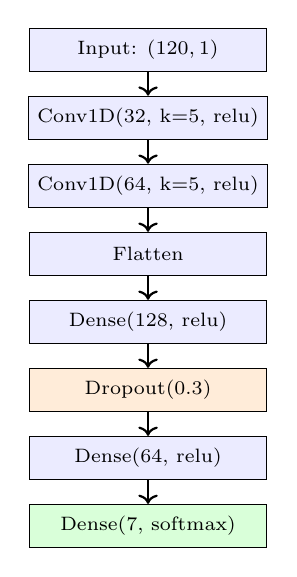
\begin{tikzpicture}[
  layer/.style={rectangle, draw, fill=blue!8, minimum width=3cm,
                minimum height=0.55cm, font=\scriptsize, align=center},
  node distance=0.3cm
]
  \node[layer] (in) {Input: $(120, 1)$};
  \node[layer, below=of in] (c1) {Conv1D(32, k=5, relu)};
  \node[layer, below=of c1] (c2) {Conv1D(64, k=5, relu)};
  \node[layer, below=of c2] (fl) {Flatten};
  \node[layer, below=of fl] (d1) {Dense(128, relu)};
  \node[layer, below=of d1, fill=orange!15] (dr) {Dropout(0.3)};
  \node[layer, below=of dr] (d2) {Dense(64, relu)};
  \node[layer, below=of d2, fill=green!15] (out) {Dense(7, softmax)};

  \draw[->, thick] (in) -- (c1);
  \draw[->, thick] (c1) -- (c2);
  \draw[->, thick] (c2) -- (fl);
  \draw[->, thick] (fl) -- (d1);
  \draw[->, thick] (d1) -- (dr);
  \draw[->, thick] (dr) -- (d2);
  \draw[->, thick] (d2) -- (out);
\end{tikzpicture}
\end{center}

\column{0.52\textwidth}
\textbf{Training details:}
\begin{itemize}
  \item Loss: sparse categorical cross-entropy
  \item Optimizer: Adam
  \item Epochs: 40 (with early stopping, patience=6)
  \item Batch size: 128
  \item LR schedule: ReduceLROnPlateau (factor=0.5)
  \item Train/val split: 80/20
\end{itemize}

\medskip
\textbf{Evaluation:}
\begin{itemize}
  \item Accuracy, confusion matrix
  \item ROC AUC (macro, one-vs-rest)
  \item PR AUC (macro)
  \item Per-class precision, recall, F1
\end{itemize}

\medskip
\textbf{Input normalization:}\\
\small StandardScaler on waveform features\\(saved as \texttt{count\_waveform\_scaler.pkl})
\end{columns}
\end{frame}

% ============================================================
\begin{frame}{Step 5: Signal Model (\texttt{train\_signal\_model.py})}
\begin{columns}[T]
\column{0.45\textwidth}
\textbf{Architecture:}
\begin{center}
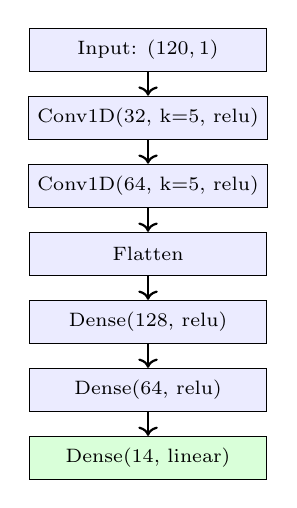
\begin{tikzpicture}[
  layer/.style={rectangle, draw, fill=blue!8, minimum width=3cm,
                minimum height=0.55cm, font=\scriptsize, align=center},
  node distance=0.3cm
]
  \node[layer] (in) {Input: $(120, 1)$};
  \node[layer, below=of in] (c1) {Conv1D(32, k=5, relu)};
  \node[layer, below=of c1] (c2) {Conv1D(64, k=5, relu)};
  \node[layer, below=of c2] (fl) {Flatten};
  \node[layer, below=of fl] (d1) {Dense(128, relu)};
  \node[layer, below=of d1] (d2) {Dense(64, relu)};
  \node[layer, below=of d2, fill=green!15] (out) {Dense(14, linear)};

  \draw[->, thick] (in) -- (c1);
  \draw[->, thick] (c1) -- (c2);
  \draw[->, thick] (c2) -- (fl);
  \draw[->, thick] (fl) -- (d1);
  \draw[->, thick] (d1) -- (d2);
  \draw[->, thick] (d2) -- (out);
\end{tikzpicture}
\end{center}

\column{0.52\textwidth}
\textbf{Output structure} (14 values):
\[
  [t_0^{(1)}, A^{(1)}, t_0^{(2)}, A^{(2)}, \ldots, t_0^{(7)}, A^{(7)}]
\]
Interleaved $t_0$ and amplitude for up to 7 signals.

\medskip
\textbf{Training details:}
\begin{itemize}
  \item Loss: MAE
  \item Optimizer: Adam
  \item Epochs: 30 (early stopping, patience=6)
  \item Batch size: 64
  \item Target normalization: separate StandardScalers for $t_0$ and $A$
\end{itemize}

\medskip
\textbf{Evaluation:}
\begin{itemize}
  \item Per-slot MAE for $t_0$ and amplitude
  \item RMSE, Pearson \& Spearman correlations
  \item Per-slot MAE bar plots
\end{itemize}
\end{columns}
\end{frame}

% ============================================================
\section{Inference \& Evaluation}

\begin{frame}{Step 6: Prediction Comparison (\texttt{compare\_signal\_predictions.py})}

\textbf{Two-stage inference:}
\begin{enumerate}
  \item Count model predicts the number of signals $\hat{n}$
  \item Signal model predicts all 14 parameters; only the first $\hat{n}$ pairs are used
\end{enumerate}

\medskip
\begin{columns}[T]
\column{0.48\textwidth}
\textbf{Metrics computed:}
\begin{itemize}
  \item $t_0$: MAE, RMSE, $R^2$, Pearson, Spearman
  \item Amplitude: MAE, RMSE, $R^2$, Pearson, Spearman
  \item Count accuracy
  \item Per-true-count breakdown
\end{itemize}

\column{0.48\textwidth}
\textbf{Plots generated:}
\begin{itemize}
  \item Hexbin: true vs predicted $t_0$
  \item Histogram: $\Delta t_0$ residuals
  \item Hexbin: true vs predicted amplitude
  \item Histogram: $\Delta A$ residuals
  \item Count model confusion matrix
\end{itemize}
\end{columns}
\end{frame}

% ============================================================
\begin{frame}{Step 7: Individual Waveform Plots}

\begin{columns}[T]
\column{0.55\textwidth}
For each waveform in the selected range:
\begin{itemize}
  \item Plot the raw (baseline-subtracted) waveform
  \item Overlay \textcolor{blue}{true} signal positions $(t_0, A)$
  \item Overlay \textcolor{green!60!black}{predicted} signal positions
  \item Predicted count determines how many markers shown
\end{itemize}

\medskip
\textbf{Batched inference:}
\begin{itemize}
  \item All predictions computed in 2 batch calls (not per-waveform)
  \item Loop only handles matplotlib plotting
  \item Default range: waveforms 1--300
\end{itemize}

\column{0.42\textwidth}
\centering
\textbf{Example output:}\\[4pt]
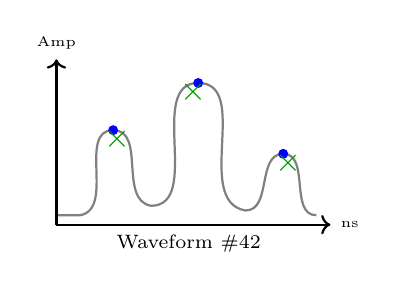
\begin{tikzpicture}[scale=0.6]
  \draw[gray, thick] (0,0.2) -- (0.5,0.2) to[out=10,in=180] (1.2,2.0)
    to[out=0,in=170] (2.0,0.4) to[out=0,in=180] (3.0,3.0)
    to[out=0,in=170] (4.0,0.3) to[out=0,in=180] (4.8,1.5)
    to[out=0,in=180] (5.5,0.2);
  \fill[blue] (1.2,2.0) circle (3pt);
  \fill[blue] (3.0,3.0) circle (3pt);
  \fill[blue] (4.8,1.5) circle (3pt);
  \node[green!60!black, font=\large] at (1.3,1.8) {$\times$};
  \node[green!60!black, font=\large] at (2.9,2.8) {$\times$};
  \node[green!60!black, font=\large] at (4.9,1.3) {$\times$};
  \draw[->, thick] (0,0) -- (5.8,0) node[right] {\tiny ns};
  \draw[->, thick] (0,0) -- (0,3.5) node[above] {\tiny Amp};
  \node[font=\scriptsize] at (2.8,-0.4) {Waveform \#42};
\end{tikzpicture}

\smallskip
\small Saved to \texttt{waveform\_inspection/}
\end{columns}
\end{frame}

% ============================================================
\section{Configuration \& CLI}

\begin{frame}[fragile]{Central Configuration (\texttt{config.py})}

All pipeline parameters in one file:

\medskip
\begin{columns}[T]
\column{0.48\textwidth}
\begin{lstlisting}[title={\scriptsize Physics \& Generation}]
TIME_START = 0        # ns
TIME_END   = 120      # ns
TAU_RISE   = 2        # ns
TAU_FALL   = 10       # ns
NUM_WAVEFORMS = 50000
NOISE_STD  = 0.5
BASELINE   = 200.0
MAX_SIGNALS = 7
\end{lstlisting}

\column{0.48\textwidth}
\begin{lstlisting}[title={\scriptsize Training \& Architecture}]
COUNT_MODEL_EPOCHS = 40
SIGNAL_MODEL_EPOCHS = 30
CONV_FILTERS = [32, 64]
CONV_KERNEL_SIZE = 5
DENSE_UNITS = [128, 64]
DROPOUT_RATE = 0.3
EARLY_STOPPING_PATIENCE = 6
\end{lstlisting}
\end{columns}

\medskip
\begin{center}
\small Edit \texttt{config.py} $\rightarrow$ all scripts pick up the changes automatically.
\end{center}
\end{frame}

% ============================================================
\begin{frame}[fragile]{CLI Usage (\texttt{cli.py})}

\textbf{Run individual steps:}
\begin{lstlisting}[language=bash]
python cli.py generate --num-waveforms 10000
python cli.py baseline
python cli.py prepare
python cli.py train-count --epochs 50
python cli.py train-signal --epochs 40
python cli.py compare
python cli.py plot --start 1 --end 50
\end{lstlisting}

\medskip
\textbf{Run the full pipeline end-to-end:}
\begin{lstlisting}[language=bash]
python cli.py run-all --experiment-name my_experiment
\end{lstlisting}

\smallskip
\begin{itemize}
  \item Steps 4 \& 5 train in \textbf{parallel} (separate processes)
  \item Results saved to timestamped \texttt{experiments/} folder with config, metrics, plots, and logs
\end{itemize}
\end{frame}

% ============================================================
\section{Performance Optimizations}

\begin{frame}{Performance Optimizations}

\begin{tabular}{@{}llll@{}}
\toprule
\textbf{Component} & \textbf{Before} & \textbf{After} & \textbf{Technique} \\
\midrule
File format & 100k+ \texttt{.txt} files & Single \texttt{.npz} per step & NumPy binary \\
Waveform gen. & Python loop (50k iter.) & Vectorized per count group & Broadcasting \\
Baseline sub. & Per-row pandas Series & Bulk DataFrame rolling & Transpose trick \\
Model training & Sequential & Parallel (2 processes) & ProcessPoolExecutor \\
Plotting & 598 predict() calls & 2 batch predict() calls & Batch inference \\
\bottomrule
\end{tabular}

\medskip
\begin{center}
\small All optimizations preserve identical numerical results.
\end{center}
\end{frame}

% ============================================================
\section{Experiment Tracking}

\begin{frame}[fragile]{Experiment Tracking}

Each \texttt{run-all} execution saves a complete experiment snapshot:

\medskip
\begin{columns}[T]
\column{0.4\textwidth}
\textbf{Folder structure:}
\begin{lstlisting}[language=bash, frame=none, backgroundcolor=\color{white}]
experiments/
  2026-03-06_02-26-12_name/
    config.json
    metrics.json
    pipeline.log
    training_plots/
    comparison_plots/
    waveform_inspection/
\end{lstlisting}

\column{0.55\textwidth}
\textbf{Contents:}
\begin{itemize}
  \item \texttt{config.json}: all CLI arguments used
  \item \texttt{metrics.json}: model metrics + per-step timings
  \item \texttt{pipeline.log}: full console log
  \item Copies of all generated plots
\end{itemize}

\medskip
\small Enables reproducible comparison across experiments with different hyperparameters.
\end{columns}
\end{frame}

% ============================================================
\begin{frame}{}
\centering
\Huge\bfseries
Thank you!

\vspace{1cm}
\large
\texttt{python cli.py run-all --experiment-name demo}
\end{frame}

\end{document}
